\chapter{Hasil dan Pembahasan}

\section{Analisis pada Sistem Operasi Linux Sungguhan}

Dengan bantuan perangkat lunak virtualisasi UTM, analisis sistem penanganan notifikasi dan sisten kontrol media pada sistem operasi Linux sungguhan dilakukan pada sebuah \textit{virtual machine} (bertindak sebagai komputer referensi) yang menjalankan sistem operasi Ubuntu 22.04 (LTS) edisi arsitektur ARM 64-bit dan berjalan di atas perangkat komputer \textit{host} MacBook Air keluaran tahun 2020 (berprosesor M1) bersistem operasi macOS 13 "Ventura".

\begin{figure}[h]
    \centering
    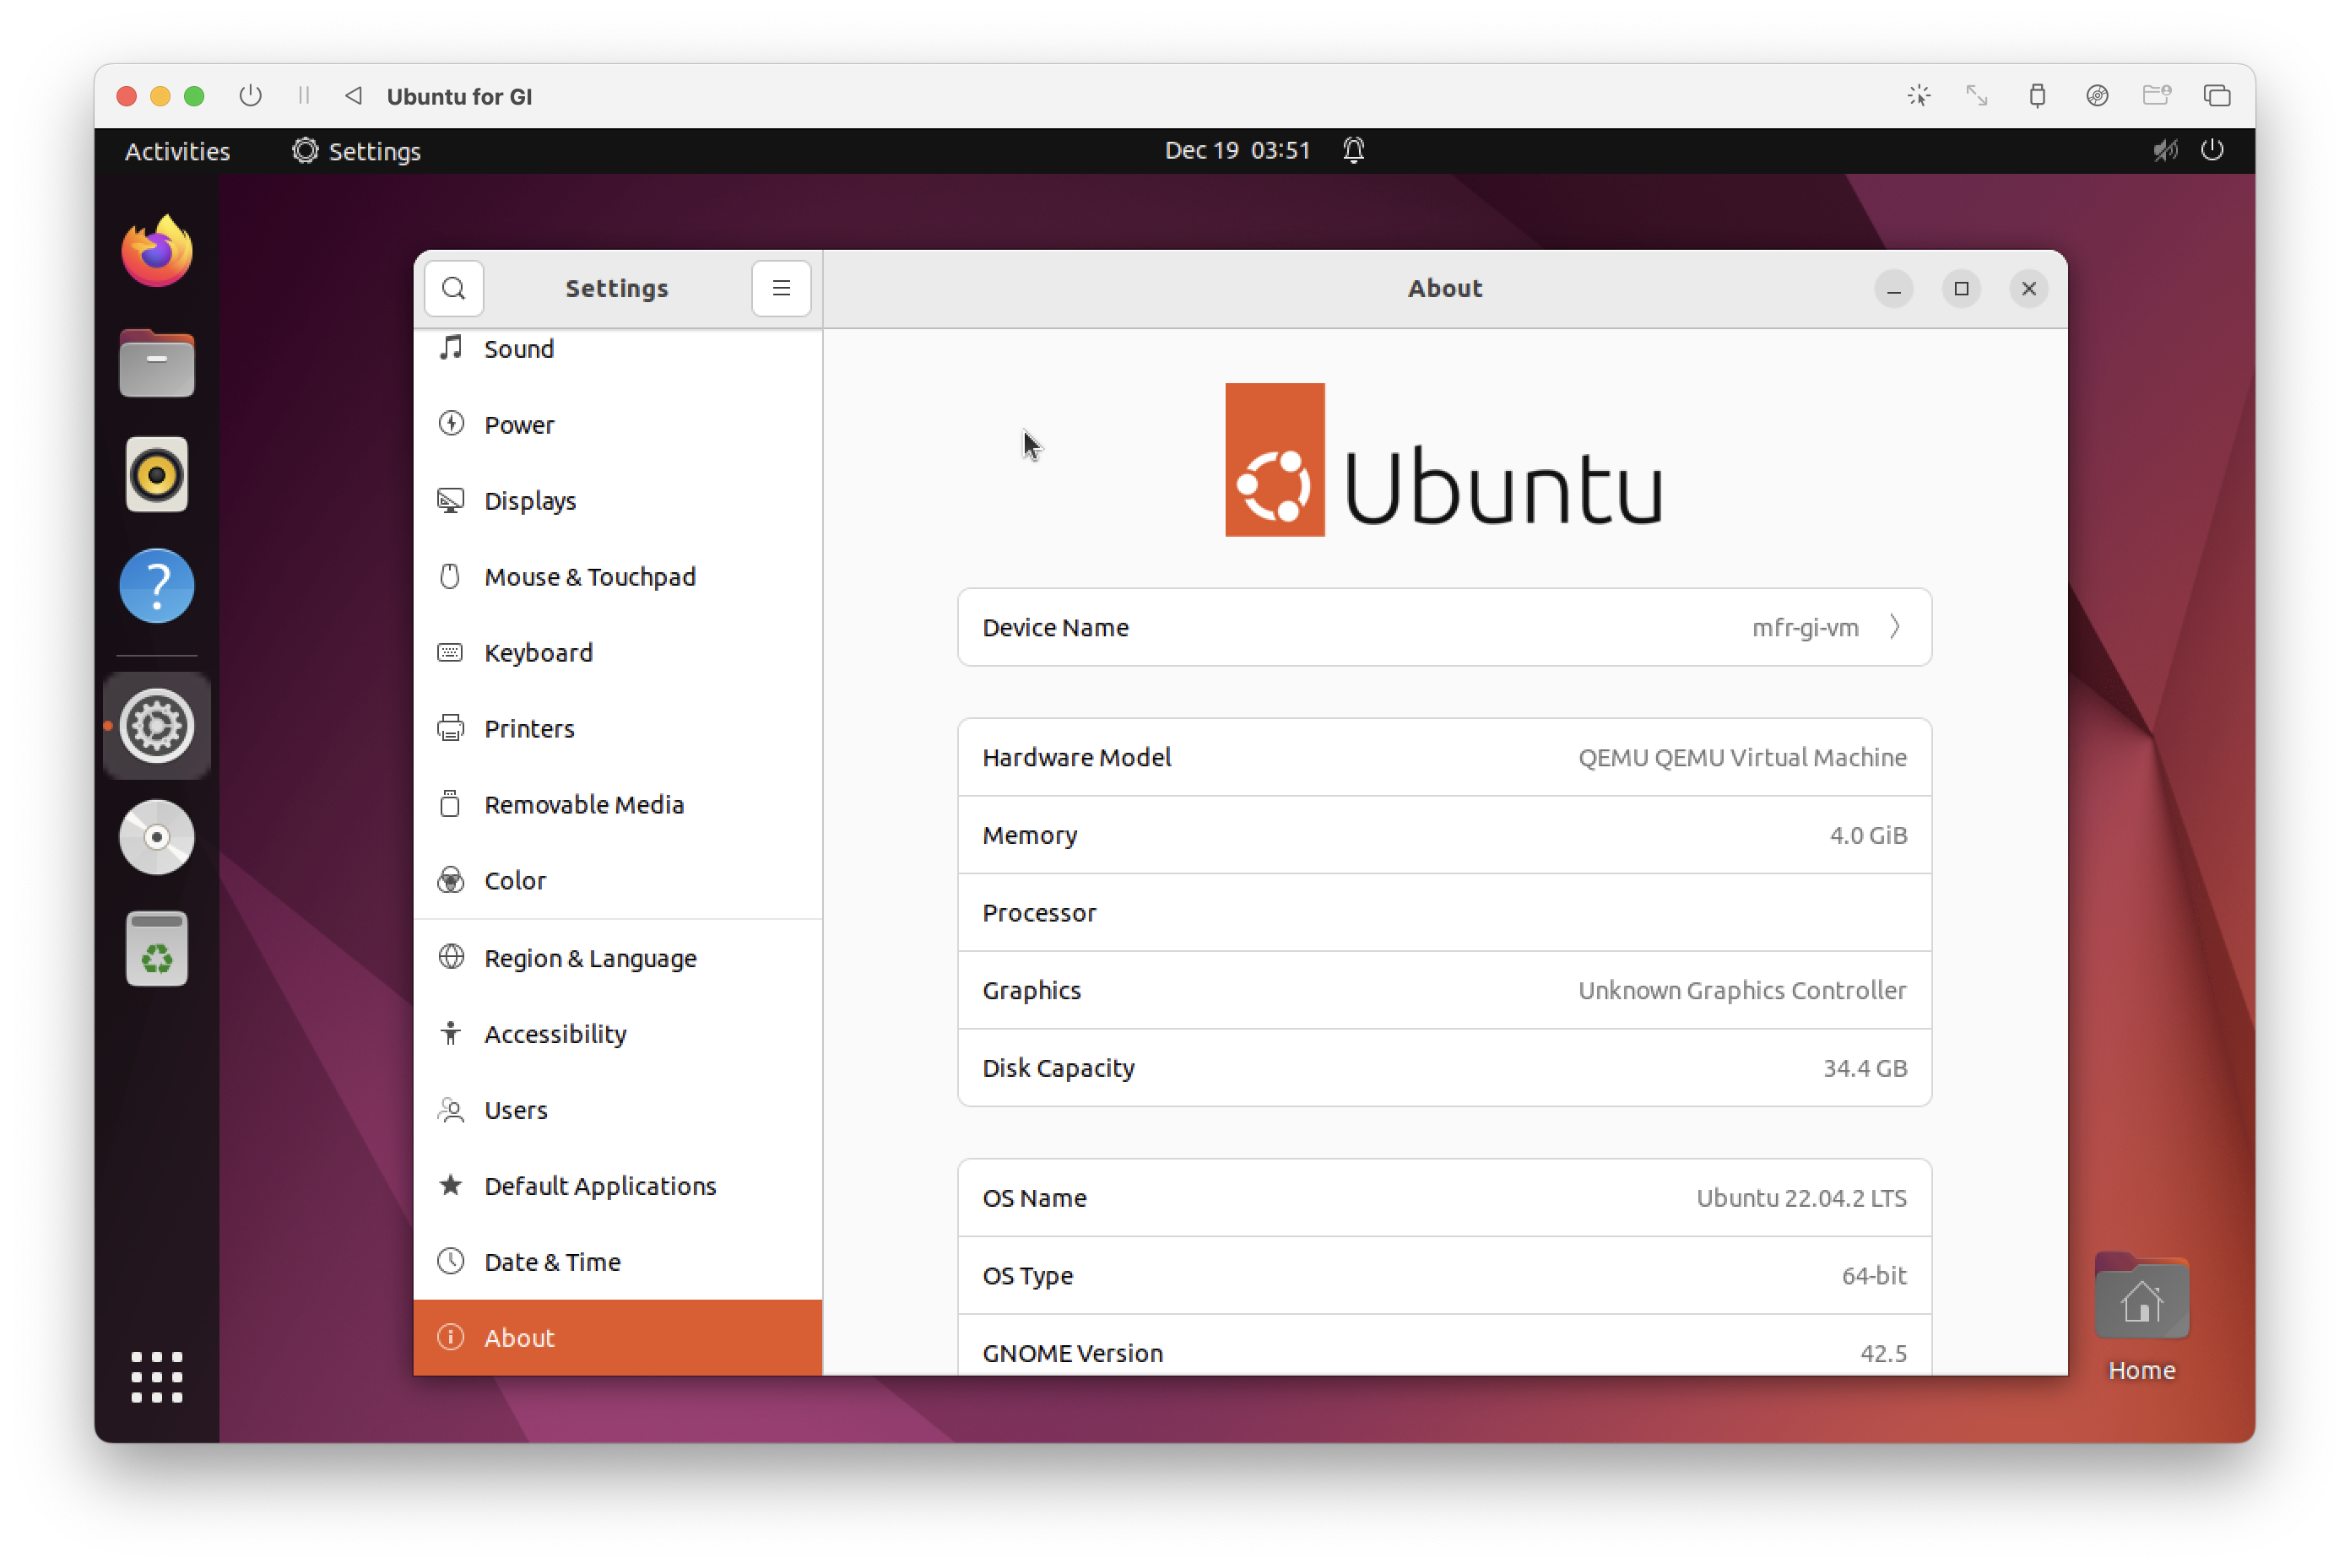
\includegraphics[width=0.75\linewidth]{archives//contents-template-pak-prapto//chapter-4/Screenshot 2023-12-19 at 10.51.04.png}
    \caption{Tangkapan layar \textit{virtual machine} Ubuntu 22.04 (LTS) yang sedang berjalan di perangkat lunak virtualisasi UTM}
    \label{fig:enter-label}
\end{figure}

\subsection{Analisis Sistem Penanganan Notifikasi}

Pengelolaan sistem penanganan notifikasi pada sistem operasi Linux bergantung pada distribusi dan/atau lingkungan desktop (\textit{desktop environment}) yang digunakan, tetapi hampir seluruh implementasi penanganan notifikasi pada sistem operasi Linux berkomunikasi melalui bus perpesanan D-Bus. Sebagai contoh, distribusi Linux yang menggunakan lingkungan \textit{desktop} GNOME menyerahkan pengelolaan notifikasi kepada \textit{desktop} GNOME itu sendiri. Uji coba sistem notifikasi pada Linux dapat dilakukan melalui berbagai cara, seperti
\begin{itemize}
    \item menggunakan perangkat lunak yang normalnya mengirimkan notifikasi (aplikasi \textit{e-mail}, aplikasi perpesanan, dan lain-lain),
    \item mensimulasikan pemanggilan metode (\textit{method}) objek D-Bus khusus yang bertugas menangani notifikasi dengan menggunakan alat (\textit{tool}) pengujian \verb|dbus-send| yang disediakan oleh paket perangkat lunak D-Bus itu sendiri, dan
    \item menggunakan alat (\textit{tool}) \verb|notify-send| yang memiliki fungsi tunggal mengirimkan notifikasi pada \textit{desktop} Linux.
\end{itemize}

Karena kepraktisannya, digunakan alat (\textit{tool}) \verb|notify-send| dalam pengujian awal ini. Alat \verb|notify-send| tersedia secara bawaan pada banyak distribusi Linux seperti Ubuntu dan Fedora. Mengutip halaman manual alat \verb|notify-send| \cite{notify-send-man-page}, alat ini dipanggil dengan bentuk pemanggilan
\begin{lstlisting}[language=bash]
    notify-send [options] {summary} [body]
\end{lstlisting}
dengan dua buah argumen utama:
\begin{itemize}
    \item argumen opsional "\textit{summary}" yang akan tertampil sebagai "judul" notifikasi dan
    \item argumen wajib "\textit{body}" yang berisi konten utama notifikasi dalam bentuk teks.
\end{itemize}
Di samping itu, alat ini juga dapat dipanggil dengan mengikutkan beberapa opsi (\textit{options}) opsional yang berkaitan dengan penampilan notifikasi:
\begin{itemize}
    \item "\verb|-u [tingkat-urgensi]|" atau "\verb|--urgency=[tingkat-urgensi]|" yang menentukan tingkat urgensi notifikasi yang akan ditampilkan (\verb|low|, \verb|normal|, atau \verb|critical|),
    \item "\verb|-t [waktu-kadaluarsa]|" atau "\verb|--expire-time=[waktu-kadaluarsa]|" yang mengatur durasi waktu notifikasi yang tertampil akan menghilang dengan sendirinya (dalam satuan milidetik),
    \item "\verb|-i [lokasi-berkas-ikon]|" atau "\verb|--icon=[lokasi-berkas-ikon]|" yang mengatur ikon yang akan ikut ditampilkan dalam notifikasi,
    \item "\verb|-c [kategori]|" atau "\verb|--category=[kategori]|" yang mengatur kategori notifikasi yang akan tertampil, dan
    \item "\verb|-h [hint]|" atau "\verb|--hint=[hint]|" yang mengatur nilai-nilai \textit{hint} untuk notifikasi yang akan tertampil.
\end{itemize}

Dalam pengujian ini, akan dikirimkan sampel notifikasi sederhana yang hanya memuat judul "Percobaan Notifikasi" dan isi pesan "Halo! Perkenalkan, nama saya Farrel.". Bentuk pemanggilan perintah \verb|notify-send| menjadi seperti berikut.
\begin{lstlisting}[language=bash]
    notify-send "Percobaan Notifikasi" "Halo! Perkenalkan, nama saya Farrel."
\end{lstlisting}
Setelah perintah tersebut dijalankan, muncul notifikasi pada layar komputer seperti pada gambar \ref{ubuntu-notify-send-demo}. Karena Ubuntu (salah satu distribusi Linux) menggunakan lingkungan desktop GNOME, penampilan notifikasi mengikuti gaya penampilan notifikasi pada lingkungan \textit{desktop} GNOME, yaitu di atas layar. Setelah beberapa saat (bergantung pada tingkat urgensi yang telah ditentukan pada pemanggilan perintah \verb|notify-send|), notifikasi akan menghilang dengan sendirinya dan masuk ke panel notifikasi yang disediakan oleh \textit{desktop} GNOME seperti pada gambar \ref{ubuntu-notification-panel}.

\begin{figure}
    \centering
    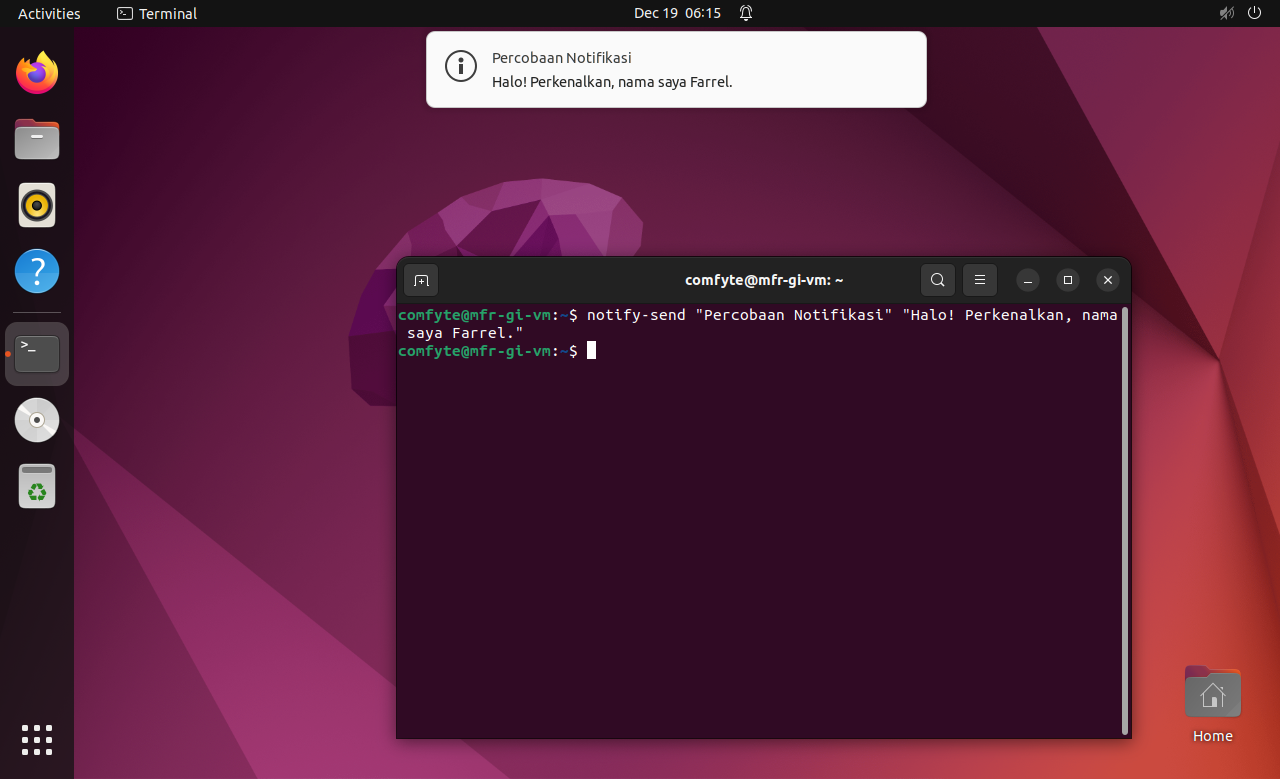
\includegraphics[width=1\linewidth]{archives//contents-template-pak-prapto//chapter-4/Screenshot from 2023-12-19 06-15-10.png}
    \caption{Notifikasi dari notify-send yang berhasil tertampil di \textit{desktop} GNOME di Ubuntu}
    \label{ubuntu-notify-send-demo}
\end{figure}

\begin{figure}
    \centering
    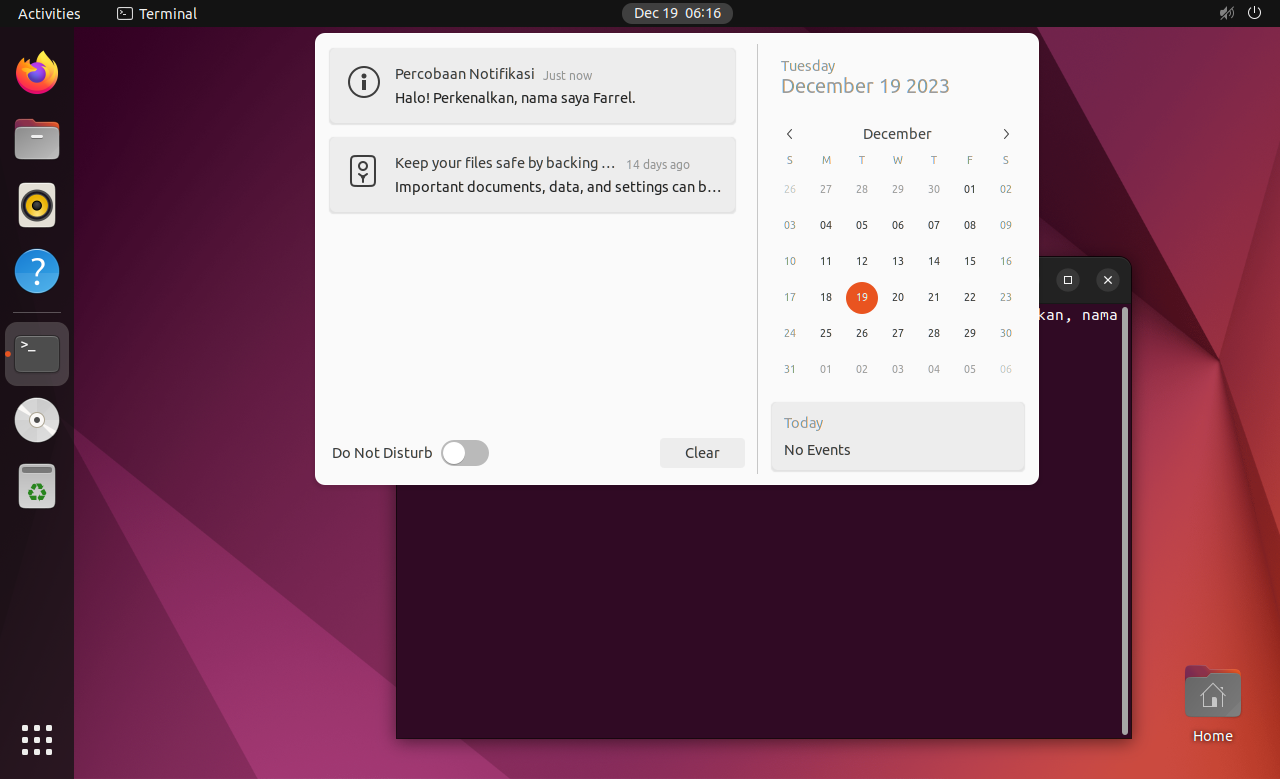
\includegraphics[width=1\linewidth]{archives//contents-template-pak-prapto//chapter-4/Screenshot from 2023-12-19 06-16-29.png}
    \caption{Panel notifikasi di \textit{desktop} GNOME yang mengumpulkan notifikasi-notifikasi lampau yang pernah tertampil}
    \label{ubuntu-notification-panel}
\end{figure}

Pada sistem operasi Linux, dimungkinkan penampilan notifikasi yang lebih kompleks (seperti mengandung tombol-tombol aksi) daripada sekadar notifikasi simpel seperti yang telah diujicobakan. Namun, mengingat alat \verb|notify-send| tidak mendukung jenis notifikasi kompleks seperti itu, pengujian pada bagian ini hanya mengujikan notifikasi yang simpel saja.

\begin{figure}
    \centering
    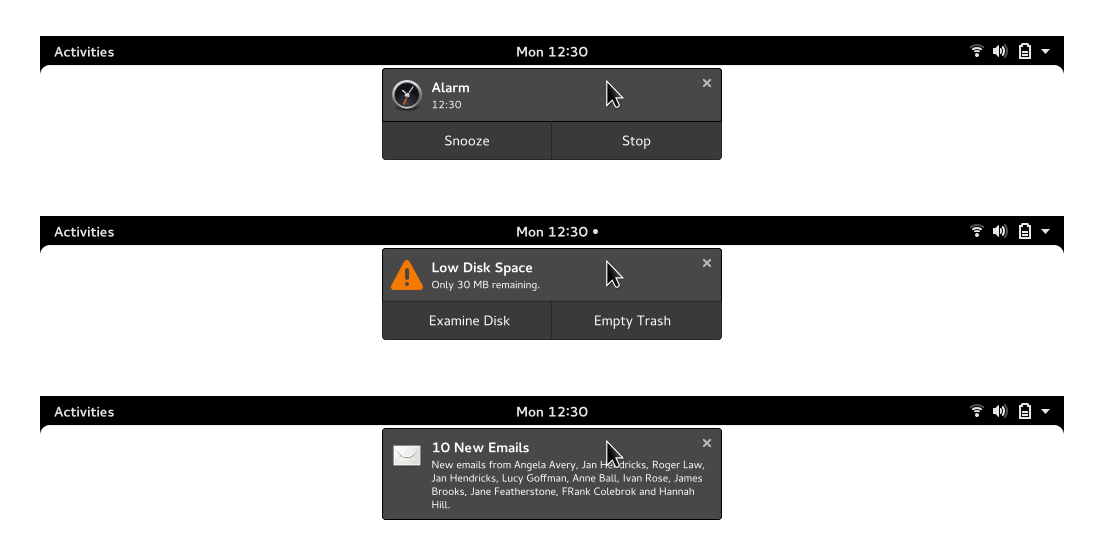
\includegraphics[width=1\linewidth]{archives//contents-template-pak-prapto//chapter-4/banners-expanded.png}
    \caption{Contoh penampilan berbagai jenis notifikasi pada lingkungan \textit{desktop} GNOME \cite{gnome-hig-notifications}; pada \textit{desktop} GNOME, notifikasi kompleks yang memiliki tombol-tombol aksi hanya akan menampilkan tombol-tombol aksi tersebut pada saat notifikasi tersebut berada di bawah kursor \textit{mouse}.}
    \label{example-of-notification-with-action-buttons-on-gnome-desktop}
\end{figure}

Di balik layar, notifikasi yang tertampil tersebut disalurkan dari \verb|notify-send| ke \textit{shell} GNOME melalui bus perpesanan D-Bus yang berjalan pada sesi (\textit{session}) pengguna saat ini. Alat \verb|notify-send| terhubung dengan bus sesi sebagai klien yang memanggil metode \verb|Notify()| pada antarmuka \verb|org.freedesktop.Notifications|; antarmuka tersebut disediakan oleh perangkat lunak \textit{notification server} yang pada lingkungan \textit{desktop} GNOME merupakan \textit{shell} GNOME itu sendiri.

Dalam serangkaian peralatan yang disediakan secara bawaan oleh paket perangkat lunak D-Bus, terdapat alat bernama \verb|dbus-monitor| yang berfungsi memantau detail pesan-pesan yang dipertukarkan di dalam bus perpesanan D-Bus. Secara \textit{default}, penjalanan \verb|dbus-monitor| tanpa memberikan argumen apa pun akan memonitor dan mencetak (di \textit{standard output}) seluruh pesan yang dipertukarkan di bus perpesanan D-Bus yang mungkin dirasa berlebihan; penjalanan \verb|dbus-monitor| dapat diatur dengan sebuah argumen yang berupa perintah filter sehingga pesan-pesan yang dimonitor dan dicetak terbatas pada pesan-pesan yang diinginkan saja. Apabila alat \verb|dbus-monitor| dijalankan dengan perintah lengkap
\begin{lstlisting}[language=bash]
    dbus-monitor "path='/org/freedesktop/Notifications'"
\end{lstlisting}
untuk memulai proses pemantauan dan perintah pengiriman notifikasi yang menggunakan \verb|notify-send| di atas dijalankan ulang, jendela terminal tempat penjalanan \verb|dbus-monitor| akan mengeluarkan informasi seperti berikut.
\begin{lstlisting}
method call time=1702972516.257275 sender=:1.48 -> destination=:1.35 serial=31 path=/org/freedesktop/Notifications; interface=org.freedesktop.Notifications; member=Notify
   string "notify-send"
   uint32 0
   string ""
   string "Percobaan Notifikasi"
   string "Halo! Perkenalkan, nama saya Farrel."
   array [
   ]
   array [
      dict entry(
         string "urgency"
         variant             byte 1
      )
      dict entry(
         string "sender-pid"
         variant             uint32 3347
      )
   ]
   int32 -1
\end{lstlisting}

Keluaran (\textit{output}) penjalanan perintah \verb|dbus-monitor| secara gamblang menunjukkan informasi-informasi teknis pada suatu penampilan notifikasi di \textit{desktop} Linux. Di samping dokumen spesifikasi resmi penanganan notifikasi di Linux sebagai acuan utama \cite{xdg-desktop-notifications-specification}, hasil keluaran ini dapat sangat bermanfaat untuk menginspeksi dan men-\textit{debug} mekanisme penanganan notifikasi pada tahap-tahap pengembangan yang dilakukan selanjutnya.

\subsection{Analisis Sistem Kontrol Media}

\section{Analisis Ekosistem pada Masing-Masing Platform (Linux dan Windows)}

\subsection{Analisis Sistem Penanganan Notifikasi}

\subsection{Analisis Sistem Kontrol Media}

\section{Pengembangan Perangkat Lunak FancyWSL}

\section{Perbandingan Hasil Penelitian dengan Hasil Terdahulu}
